Die Keplergleichung wird in der Himmelsmechanik gebraucht, um die 
Position von Planeten und Satellition in Abh"angigkeit von der Zeit
zu berechnen, die sich auf elliptischen Bahnen bewegen.
Zu gegebenem $M$ ist die Zahl $E$ zu finden, f"ur die die Gleichung
\[
E-e\sin E=M
\]
gilt.
Die Zahl $e$ ist die Exzentrizit"at der Ellipsenbahn. F"ur $e=0$
geht die Ellipse in einen Kreis "uber, und die Gleichung ist trivial
zu l"osen. Finden sie eine St"orungsl"osung vierter Ordnung
der Kepler-Gleichung in Abh"angigkeit von $e$ als St"orungsparameter.

\begin{loesung}
Wir setzen $E$ als Funktion von $e$ an
\[
E(e)
=
E_0+E_1e+E_2e^2+\dots
\]
Dies setzen wir in die Keplergleichung ein
\begin{align*}
M
&=
E(e)-e\sin E(e)
\\
&=
E_0+E_1e+E_2e^2+\dots
-e\biggl(
E(e)-\frac1{3!}E(e)^3+\dots
\biggr)
\\
&=
E_0+E_1e+E_2e^2+E_3e^3+E_4e^4+\dots
-e\biggl(
E_0+E_1e+E_2e^2+E_3e^3+E_4e^4+\dots
-E_0^3e^3-\dots
\biggr)
\end{align*}
weitere Terme auf der rechten Seite m"ussen nicht ber"ucksichtigt
werden, weil sie h"ohere Ordnung als 4 haben.
Es bleibt also die Gleichung
\begin{align*}
M
&=
E_0+E_1e+E_2e^2+E_3e^3+E_4e^4
-E_0e-E_1e^2-E_2e^3-E_3e^4
+E_0^3e^4+\dots
\\
&=
E_0
+(E_1-E_0)e
+(E_2-E_1)e^2
+(E_3-E_2)e^3
+(E_4-E_3+E_0^3)e^4
\end{align*}
Aus dem Koeffizientenvergleich k"onnen wir jetzt die Koeffizienten ablesen
\begin{equation}
\begin{aligned}
E_0&=M
\\
E_1-E_0&=0&&\Rightarrow&E_1&=E_0=M\\
E_2-E_1&=0&&\Rightarrow&E_2&=E_1=M\\
E_3-E_2&=0&&\Rightarrow&E_3&=E_2=M\\
E_4-E_3+E_0^3&=0&&\Rightarrow&E_4&=E_3-E_0^3=M-M^3
\end{aligned}
\end{equation}
Die St"orungsreihe bis zur vierten Ordnung f"ur $E$ ist also
\[
E(e)=M+Me+Me^2+Me^3+(M-M^3)e^4.
\]
\begin{figure}
\centering
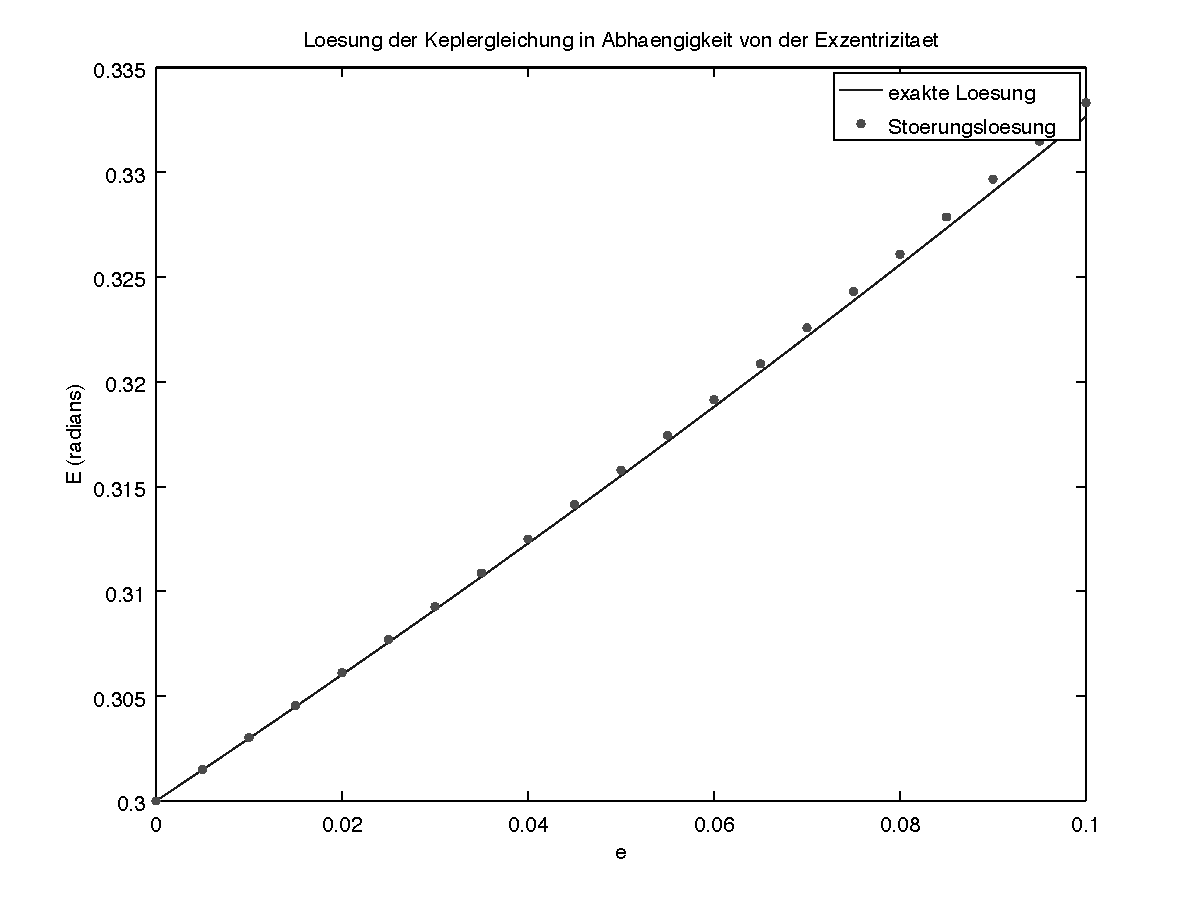
\includegraphics[width=\hsize]{uebungsaufgaben/kepler.pdf}
\caption{St"orungsl"osung der Kepler-Gleichung f"ur $M=0.3$
\label{10001:kepler}}
\end{figure}
Ein Vergleich der exakten L"osung mit der St"orungsl"osung findet sich
in Abbildung~\ref{10001:kepler}.
\end{loesung}

